% Source PDF page 55 (printed p. 41)
$\theta t+(1-\theta)s>0$ 显然成立。上述结论由下式得到：
\[
 \frac{\theta x+(1-\theta)y}{\theta t+(1-\theta)s}
 =\mu(x/t)+(1-\mu)(y/s),
 \qquad\mu=\frac{\theta t}{\theta t+(1-\theta)s}\in[0,1].
\]

\subsubsection*{线性分式函数}
将透视函数与仿射函数复合，得到\emph{线性分式函数}。设 $g:\R^n\to\R^{m+1}$ 为仿射函数，即
\begin{equation}
 g(x)=\begin{bmatrix}A\\c^{\T}\end{bmatrix}x+
 \begin{bmatrix}b\\d\end{bmatrix},\tag{2.12}
\end{equation}
其中 $A\in\R^{m\times n}$、$b\in\R^m$、$c\in\R^n$、$d\in\R$。由 $f=P\circ g$ 定义的函数 $f:\R^n\to\R^m$，即
\begin{equation}
 f(x)=(Ax+b)/(c^{\T}x+d),\qquad
 \dom f=\{x\mid c^{\T}x+d>0\},\tag{2.13}
\end{equation}
称为\emph{线性分式函数}或\emph{射影函数}。当 $c=0$、$d>0$ 时，$\dom f=\R^n$，且 $f$ 为仿射函数。因此，可以把仿射函数和线性函数视为线性分式函数的特例。

\begin{quote}\textbf{说明2.2\quad 射影解释。}
将线性分式函数表示为矩阵
\begin{equation}
 Q=\begin{bmatrix}A&b\\c^{\T}&d\end{bmatrix}
 \in\R^{(m+1)\times(n+1)}\tag{2.14}
\end{equation}
往往很方便。它作用于，即乘上，形如 $(x,1)$ 的点，得到 $(Ax+b,c^{\T}x+d)$。然后将结果缩放或归一化，使最后一个分量为一，得到 $(f(x),1)$。

这个表示可以通过将 $\R^n$ 与 $\R^{n+1}$ 中的一组射线关联起来，获得几何解释。对每个 $z\in\R^n$，关联 $\R^{n+1}$ 中的开射线 $\mathcal P(z)=\{t(z,1)\mid t>0\}$。该射线的最后一个分量取正值。反过来，$\R^{n+1}$ 中任意以原点为基点、最后一个分量取正值的射线，都能对某个 $v\in\R^n$ 写成 $\mathcal P(v)=\{t(v,1)\mid t\ge0\}$。$\R^n$ 与最后一个分量为正的半空间中各射线之间的这一射影对应 $\mathcal P$，是双射。

线性分式函数（2.13）可写成
\[
 f(x)=\mathcal P^{-1}(Q\mathcal P(x)).
\]
因此，从 $x\in\dom f$，即 $c^{\T}x+d>0$ 出发，先在 $\R^{n+1}$ 中形成射线 $\mathcal P(x)$；矩阵 $Q$ 对应的线性变换将该射线变为另一条射线 $Q\mathcal P(x)$。因为 $x\in\dom f$，新射线的最后一个分量取正值。最后，作逆射影变换得到 $f(x)$。
\end{quote}

% Source PDF page 56 (printed p. 42)
\begin{figure}[htbp]\centering
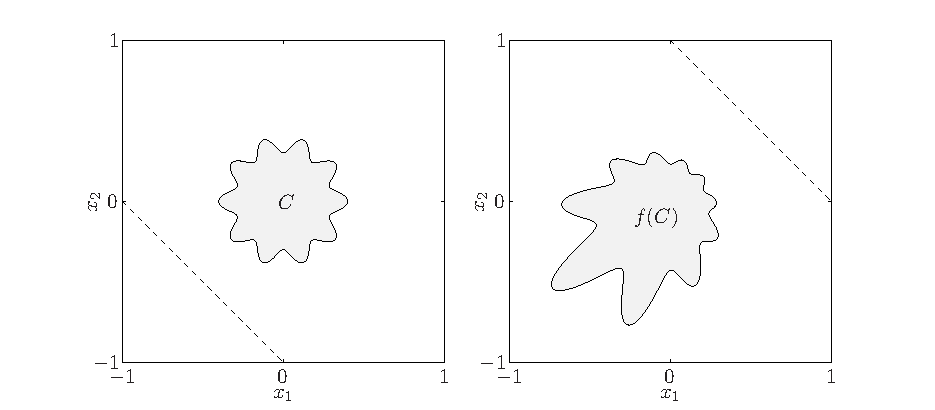
\includegraphics[width=.88\textwidth]{figures/ch02-figure-16.pdf}
\caption*{图2.16\quad 左：集合 $C\subseteq\R^2$。虚线表示线性分式函数 $f(x)=x/(x_1+x_2+1)$ 的定义域边界，其中 $\dom f=\{(x_1,x_2)\mid x_1+x_2+1>0\}$。右：$C$ 在 $f$ 下的像。虚线表示 $f^{-1}$ 的定义域边界。}
\end{figure}
与透视函数一样，线性分式函数保持凸性。如果 $C$ 凸且在 $f$ 的定义域内，即对 $x\in C$ 有 $c^{\T}x+d>0$，则其像 $f(C)$ 凸。这由前面的结果直接得到：$C$ 在仿射映射（2.12）下的像凸，这个像再经透视函数 $P$ 映射得到 $f(C)$，仍凸。类似地，若 $C\subseteq\R^m$ 凸，则逆像 $f^{-1}(C)$ 凸。

\begin{origexample}{2.13}
\textbf{条件概率。}设随机变量 $u$ 和 $v$ 分别取值于 $\{1,\ldots,n\}$ 和 $\{1,\ldots,m\}$，用 $p_{ij}$ 表示 $\Prob(u=i,v=j)$。条件概率 $f_{ij}=\Prob(u=i\mid v=j)$ 为
\[
 f_{ij}=\frac{p_{ij}}{\sum_{k=1}^n p_{kj}}.
\]
因此，$f$ 由 $p$ 经线性分式映射得到。

由此可知，如果 $C$ 是 $(u,v)$ 的联合概率构成的凸集，那么相应的给定 $v$ 时 $u$ 的条件概率集合也凸。
\end{origexample}
图2.16给出集合 $C\subseteq\R^2$ 及其在线性分式函数
\[
 f(x)=\frac1{x_1+x_2+1}x,\qquad
 \dom f=\{(x_1,x_2)\mid x_1+x_2+1>0\}
\]
下的像。

% Source PDF page 57 (printed p. 43)
\section{广义不等式}
\subsection{正常锥与广义不等式}
如果锥 $K\subseteq\R^n$ 满足以下条件，就称其为\emph{正常锥}：
\begin{itemize}
\item $K$ 凸。
\item $K$ 闭。
\item $K$ 是实心的，即内部非空。
\item $K$ 尖，即不包含直线，等价地，$x\in K$、$-x\in K$ 蕴含 $x=0$。
\end{itemize}
正常锥 $K$ 可以用来定义\emph{广义不等式}，它是 $\R^n$ 上的一种偏序，具有 $\R$ 上通常次序的许多性质。与正常锥 $K$ 关联的偏序定义为
\[
 x\preceq_K y\quad\Longleftrightarrow\quad y-x\in K.
\]
也用 $x\succeq_K y$ 表示 $y\preceq_K x$。类似地，定义相应的严格偏序
\[
 x\prec_K y\quad\Longleftrightarrow\quad y-x\in\operatorname{int}K,
\]
用 $x\succ_K y$ 表示 $y\prec_K x$。为区别于严格广义不等式 $\prec_K$，有时将 $\preceq_K$ 称为非严格广义不等式。

当 $K=\R_+$ 时，偏序 $\preceq_K$ 就是 $\R$ 上通常的次序 $\le$，严格偏序 $\prec_K$ 就是通常的严格次序 $<$。因此，广义不等式包含 $\R$ 中普通的非严格与严格不等式这一特例。

\begin{origexample}{2.14}
\textbf{非负正交锥与逐分量不等式。}非负正交锥 $K=\R_+^n$ 是正常锥。相应的广义不等式 $\preceq_K$ 对应向量间的逐分量不等式：$x\preceq_K y$ 表示 $x_i\le y_i$，$i=1,\ldots,n$。相应的严格不等式对应逐分量严格不等式：$x\prec_K y$ 表示 $x_i<y_i$，$i=1,\ldots,n$。

与非负正交锥关联的非严格与严格偏序经常出现，因此省略下标 $\R_+^n$；当符号 $\preceq$ 或 $\prec$ 出现在向量之间时，就按此理解。
\end{origexample}

\begin{origexample}{2.15}
\textbf{半正定锥与矩阵不等式。}半正定锥 $\mathbf S_+^n$ 是 $\mathbf S^n$ 中的正常锥。相应的广义不等式 $\preceq_K$ 就是通常的矩阵不等式：$X\preceq_K Y$ 表示 $Y-X$ 半正定。$\mathbf S_+^n$ 在 $\mathbf S^n$ 中的内部由正定矩阵构成，因此严格广义不等式也与对称矩阵间通常的严格不等式一致：$X\prec_K Y$ 表示 $Y-X$ 正定。

这一偏序也十分常见，因此同样省略下标，对对称矩阵只写 $X\preceq Y$ 或 $X\prec Y$，并理解为相对于半正定锥的广义不等式。
\end{origexample}

% Source PDF page 58 (printed p. 44)
\begin{origexample}{2.16}
\textbf{在 $[0,1]$ 上非负的多项式锥。}定义
\begin{equation}
 K=\{c\in\R^n\mid c_1+c_2t+\cdots+c_nt^{n-1}\ge0,\ t\in[0,1]\}.\tag{2.15}
\end{equation}
即 $K$ 是在区间 $[0,1]$ 上非负的 $n-1$ 次多项式的系数构成的锥。可以证明，$K$ 是正常锥；其内部是在区间 $[0,1]$ 上为正的多项式的系数集。

两个向量 $c,d\in\R^n$ 满足 $c\preceq_K d$，当且仅当对所有 $t\in[0,1]$ 有
\[
 c_1+c_2t+\cdots+c_nt^{n-1}
 \le d_1+d_2t+\cdots+d_nt^{n-1}.
\]
\end{origexample}

\subsubsection*{广义不等式的性质}
广义不等式 $\preceq_K$ 满足许多性质，例如：
\begin{itemize}
\item 加法保持 $\preceq_K$：若 $x\preceq_K y$、$u\preceq_K v$，则 $x+u\preceq_K y+v$。
\item 传递性：若 $x\preceq_K y$、$y\preceq_K z$，则 $x\preceq_K z$。
\item 非负缩放保持 $\preceq_K$：若 $x\preceq_K y$、$\alpha\ge0$，则 $\alpha x\preceq_K\alpha y$。
\item 自反性：$x\preceq_K x$。
\item 反对称性：若 $x\preceq_K y$ 且 $y\preceq_K x$，则 $x=y$。
\item 取极限保持 $\preceq_K$：若对 $i=1,2,\ldots$ 有 $x_i\preceq_K y_i$，且 $i\to\infty$ 时 $x_i\to x$、$y_i\to y$，则 $x\preceq_K y$。
\end{itemize}
相应的严格广义不等式 $\prec_K$ 满足例如以下性质：
\begin{itemize}
\item 若 $x\prec_K y$，则 $x\preceq_K y$。
\item 若 $x\prec_K y$、$u\preceq_K v$，则 $x+u\prec_K y+v$。
\item 若 $x\prec_K y$、$\alpha>0$，则 $\alpha x\prec_K\alpha y$。
\item $x\not\prec_K x$。
\item 若 $x\prec_K y$，则对足够小的 $u$ 和 $v$，有 $x+u\prec_K y+v$。
\end{itemize}
这些性质来自 $\preceq_K$、$\prec_K$ 的定义及正常锥的性质，见习题2.30。

% Source PDF page 59 (printed p. 45)
\subsection{最小元与极小元}
广义不等式的记号 $\preceq_K$、$\prec_K$ 意在提示其与 $\R$ 上普通不等式 $\le$、$<$ 的类比。虽然普通不等式的许多性质对广义不等式成立，但一些重要性质并不成立。最明显的区别是，$\R$ 上的 $\le$ 是全序：任意两点都可比较，即 $x\le y$ 或 $y\le x$ 总有一个成立。其他广义不等式不具备这一性质。一个后果是，最小值与最大值等概念在广义不等式下会更复杂。本节简要讨论这一点。

若 $x\in S$，且对每个 $y\in S$ 都有 $x\preceq_K y$，就称 $x$ 为 $S$ 关于广义不等式 $\preceq_K$ 的\emph{最小元}。类似地，可以定义集合 $S$ 关于广义不等式的\emph{最大元}。如果集合有最小元或最大元，它就是唯一的。另一个相关概念是\emph{极小元}：若 $x\in S$，且 $y\in S$、$y\preceq_K x$ 只有在 $y=x$ 时才成立，就称 $x$ 为 $S$ 关于 $\preceq_K$ 的极小元。\emph{极大元}的定义类似。一个集合可以有许多不同的极小元或极大元。

可用简单的集合记号描述最小元与极小元。点 $x\in S$ 是 $S$ 的最小元，当且仅当
\[
 S\subseteq x+K.
\]
这里 $x+K$ 表示所有能与 $x$ 比较、且按照 $\preceq_K$ 大于或等于 $x$ 的点。点 $x\in S$ 是极小元，当且仅当
\[
 (x-K)\cap S=\{x\}.
\]
这里 $x-K$ 表示所有能与 $x$ 比较、且按照 $\preceq_K$ 小于或等于 $x$ 的点；它与 $S$ 唯一的公共点为 $x$。

当 $K=\R_+$ 时，诱导的就是 $\R$ 上通常的次序，极小元与最小元概念相同，都与通常的集合最小元定义一致。

\begin{origexample}{2.17}
考虑诱导 $\R^2$ 中逐分量不等式的锥 $\R_+^2$。此时，最小元与极小元具有简单的几何描述。不等式 $x\preceq y$ 表示 $y$ 位于 $x$ 的右上方。说 $x\in S$ 是集合 $S$ 的最小元，就是说 $S$ 中所有其他点都位于它的右上方。说 $x$ 是 $S$ 的极小元，就是说 $S$ 中没有其他点位于 $x$ 的左下方，如图2.17所示。
\end{origexample}

\begin{origexample}{2.18}
\textbf{对称矩阵集合的最小元与极小元。}对每个 $A\in\mathbf S_{++}^n$，关联以原点为中心的椭球
\[
 \mathcal E_A=\{x\mid x^{\T}A^{-1}x\le1\}.
\]
$A\preceq B$ 当且仅当 $\mathcal E_A\subseteq\mathcal E_B$。

给定 $v_1,\ldots,v_k\in\R^n$，定义
\[
 S=\{P\in\mathbf S_{++}^n\mid v_i^{\T}P^{-1}v_i\le1,\ i=1,\ldots,k\}.
\]
这个集合对应所有包含 $v_1,\ldots,v_k$ 的椭球。$S$ 没有最小元：对任意一个包含这些点的椭球，总能找到另一个也包含这些点、但与之不可比较的椭球。若某个椭球包含这些点，而任何更小的椭球都无法包含它们，则该椭球是极小的。图2.18给出了 $\R^2$ 中 $k=2$ 的一个例子。
\end{origexample}

% Source PDF page 60 (printed p. 46)
\begin{figure}[htbp]\centering
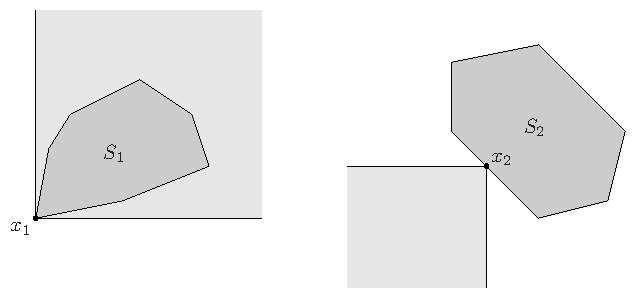
\includegraphics[width=.82\textwidth]{figures/ch02-figure-17.pdf}
\caption*{图2.17\quad 左：集合 $S_1$ 关于 $\R^2$ 中逐分量不等式有最小元 $x_1$。$x_1+K$ 以浅色阴影表示；由于 $S_1\subseteq x_1+K$，$x_1$ 是最小元。右：$x_2$ 是 $S_2$ 的极小点。$x_2-K$ 以浅色阴影表示；因为 $x_2-K$ 与 $S_2$ 仅在 $x_2$ 处相交，所以 $x_2$ 为极小点。}
\end{figure}

\section{分离超平面与支撑超平面}
\subsection{分离超平面定理}
本节介绍一个在后面十分重要的思想：用超平面或仿射函数分离不相交的凸集。基本结果是\emph{分离超平面定理}：设 $C$ 和 $D$ 为非空、不相交的凸集，即 $C\cap D=\varnothing$。那么存在 $a\ne0$ 和 $b$，使对所有 $x\in C$ 有 $a^{\T}x\le b$，对所有 $x\in D$ 有 $a^{\T}x\ge b$。换言之，仿射函数 $a^{\T}x-b$ 在 $C$ 上非正，在 $D$ 上非负。超平面 $\{x\mid a^{\T}x=b\}$ 称为集合 $C$ 和 $D$ 的\emph{分离超平面}，或称它\emph{分离}了 $C$ 和 $D$，见图2.19。

\subsubsection*{分离超平面定理的证明}
这里考虑一个特殊情形，一般情形的证明留作习题2.22。假设 $C$ 与 $D$ 的欧几里得距离
\[
 \dist(C,D)=\inf\{\norm{u-v}_2\mid u\in C,\ v\in D\}
\]
为正，而且存在 $c\in C$、$d\in D$ 取到这个最小距离，即 $\norm{c-d}_2=\dist(C,D)$。例如，$C$、$D$ 都闭且其中一个有界时，这些条件成立。

% Source PDF page 61 (printed p. 47)
\begin{figure}[htbp]\centering
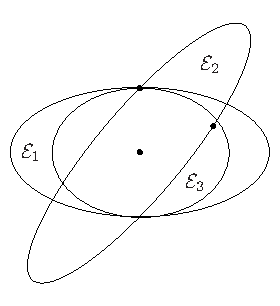
\includegraphics[width=.67\textwidth]{figures/ch02-figure-18.pdf}
\caption*{图2.18\quad $\R^2$ 中三个以原点（下方实点）为中心、包含上方各实点的椭球。$\mathcal E_1$ 不是极小的，因为存在更小、且仍包含这些点的椭球，例如 $\mathcal E_3$；$\mathcal E_3$ 也因同样理由不是极小的。$\mathcal E_2$ 是极小的，因为不存在另一个以原点为中心、包含这些点且包含于 $\mathcal E_2$ 中的椭球。}
\end{figure}
\begin{figure}[htbp]\centering
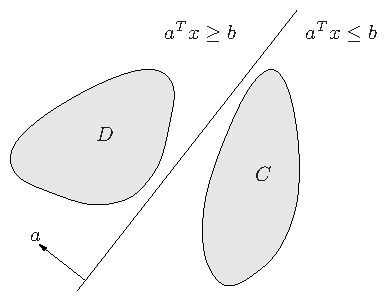
\includegraphics[width=.67\textwidth]{figures/ch02-figure-19.pdf}
\caption*{图2.19\quad 超平面 $\{x\mid a^{\T}x=b\}$ 分离了不相交的凸集 $C$ 和 $D$。仿射函数 $a^{\T}x-b$ 在 $C$ 上非正，在 $D$ 上非负。}
\end{figure}

% Source PDF page 62 (printed p. 48)
\begin{figure}[htbp]\centering
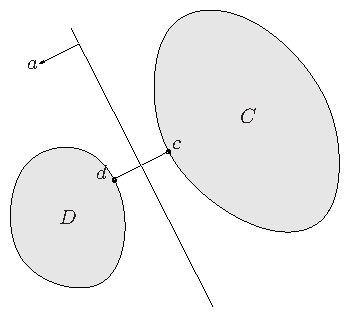
\includegraphics[width=.65\textwidth]{figures/ch02-figure-20.pdf}
\caption*{图2.20\quad 两个凸集之间分离超平面的构造。$c\in C$、$d\in D$ 是两个集合中彼此距离最近的一对点。分离超平面垂直平分 $c$ 与 $d$ 之间的线段。}
\end{figure}
定义
\[
 a=d-c,\qquad b=\frac{\norm d_2^2-\norm c_2^2}{2}.
\]
我们将证明，仿射函数
\[
 f(x)=a^{\T}x-b=(d-c)^{\T}\bigl(x-(1/2)(d+c)\bigr)
\]
在 $C$ 上非正，在 $D$ 上非负，即超平面 $\{x\mid a^{\T}x=b\}$ 分离 $C$ 与 $D$。如图2.20所示，这个超平面与线段 $cd$ 垂直，且经过其中点。

先证明 $f$ 在 $D$ 上非负。$f$ 在 $C$ 上非正的证明类似，也可以交换 $C$ 与 $D$ 并考虑 $-f$ 得到。假设存在 $u\in D$，使
\begin{equation}
 f(u)=(d-c)^{\T}\bigl(u-(1/2)(d+c)\bigr)<0.\tag{2.16}
\end{equation}
可将 $f(u)$ 写成
\[
\begin{aligned}
 f(u)&=(d-c)^{\T}\bigl(u-d+(1/2)(d-c)\bigr)\\
 &=(d-c)^{\T}(u-d)+(1/2)\norm{d-c}_2^2.
\end{aligned}
\]
因此，（2.16）蕴含 $(d-c)^{\T}(u-d)<0$。又有
\[
 \left.\frac{\mathrm d}{\mathrm dt}\norm{d+t(u-d)-c}_2^2\right|_{t=0}
 =2(d-c)^{\T}(u-d)<0,
\]
所以存在足够小的 $t>0$，且 $t\le1$，使
\[
 \norm{d+t(u-d)-c}_2<\norm{d-c}_2.
\]

% Source PDF page 63 (printed p. 49)
也就是说，$d+t(u-d)$ 比 $d$ 更接近 $c$。由于 $D$ 凸，且包含 $d$ 和 $u$，有 $d+t(u-d)\in D$。但这不可能，因为已经假设 $d$ 是 $D$ 中距 $C$ 最近的点。

\begin{origexample}{2.19}
\textbf{仿射集与凸集的分离。}设 $C$ 凸，$D$ 仿射，即 $D=\{Fu+g\mid u\in\R^m\}$，其中 $F\in\R^{n\times m}$。若 $C$、$D$ 不相交，则由分离超平面定理，存在 $a\ne0$ 和 $b$，使 $C$ 上有 $a^{\T}x\le b$，$D$ 上有 $a^{\T}x\ge b$。

条件 $a^{\T}x\ge b$ 对所有 $x\in D$ 成立，意味着 $a^{\T}Fu\ge b-a^{\T}g$ 对所有 $u\in\R^m$ 成立。但线性函数在整个 $\R^m$ 上有下界，只有当其恒为零时才可能。因此 $a^{\T}F=0$，进而 $b\le a^{\T}g$。

综上，存在 $a\ne0$，使 $F^{\T}a=0$，且对所有 $x\in C$ 有 $a^{\T}x\le a^{\T}g$。
\end{origexample}

\subsubsection*{严格分离}
上面构造的分离超平面满足更强的条件：对所有 $x\in C$，$a^{\T}x<b$；对所有 $x\in D$，$a^{\T}x>b$。这称为集合 $C$ 和 $D$ 的\emph{严格分离}。简单例子表明，一般情况下，不相交的凸集未必能被一个超平面严格分离，即使两者都闭也如此，见习题2.23。但在许多特殊情形下，可以证明严格分离成立。

\begin{origexample}{2.20}
\textbf{一点与闭凸集的严格分离。}设 $C$ 为闭凸集，$x_0\notin C$，则存在一个超平面将 $x_0$ 与 $C$ 严格分离。

为证明这一点，注意到存在 $\epsilon>0$，使 $C$ 与 $B(x_0,\epsilon)$ 不相交。由分离超平面定理，存在 $a\ne0$ 和 $b$，使 $x\in C$ 时 $a^{\T}x\le b$，$x\in B(x_0,\epsilon)$ 时 $a^{\T}x\ge b$。

利用 $B(x_0,\epsilon)=\{x_0+u\mid\norm u_2\le\epsilon\}$，第二个条件可写为
\[
 a^{\T}(x_0+u)\ge b,\qquad\text{对所有 }\norm u_2\le\epsilon.
\]
使左边最小的 $u$ 是 $u=-\epsilon a/\norm a_2$，代入得
\[
 a^{\T}x_0-\epsilon\norm a_2\ge b.
\]
因此，仿射函数
\[
 f(x)=a^{\T}x-b-\epsilon\norm a_2/2
\]
在 $C$ 上为负，在 $x_0$ 处为正。

这还立即证明了前面提到的事实：闭凸集是所有包含它的半空间的交。事实上，设 $C$ 闭且凸，$S$ 为所有包含 $C$ 的半空间之交。显然，$x\in C$ 蕴含 $x\in S$。反过来，假设存在 $x\in S$、$x\notin C$。由严格分离的结果，存在超平面严格分离 $x$ 与 $C$，即存在一个包含 $C$ 但不包含 $x$ 的半空间。换言之，$x\notin S$。
\end{origexample}

% Source PDF page 64 (printed p. 50)
\subsubsection*{逆分离超平面定理}
分离超平面定理的逆命题，即存在分离超平面就蕴含 $C$ 和 $D$ 不相交，并不成立，除非在凸性之外，对 $C$ 或 $D$ 施加额外条件。一个简单反例是 $C=D=\{0\}\subseteq\R$，超平面 $x=0$ 分离了 $C$ 和 $D$。

通过增加关于 $C$ 和 $D$ 的条件，可以得到各种逆分离定理。一个非常简单的例子是：设 $C$、$D$ 凸，且 $C$ 开；若存在仿射函数 $f$，使它在 $C$ 上非正、在 $D$ 上非负，则 $C$ 和 $D$ 不相交。为说明这一点，先注意到 $f$ 在 $C$ 上必为负；若 $f$ 在 $C$ 中某点为零，就会在该点附近取正值，从而矛盾。由于 $f$ 在 $C$ 上为负、在 $D$ 上非负，$C$ 与 $D$ 必不相交。将这个逆命题与分离超平面定理结合，得到：任意两个凸集 $C$ 和 $D$，若至少一个开，则它们不相交，当且仅当存在分离超平面。

\begin{origexample}{2.21}
\textbf{严格线性不等式的择一定理。}我们推导严格线性不等式组
\begin{equation}
 Ax\prec b\tag{2.17}
\end{equation}
有解的充要条件。这组不等式不可行，当且仅当两个凸集
\[
 C=\{b-Ax\mid x\in\R^n\},\qquad
 D=\R_{++}^m=\{y\in\R^m\mid y\succ0\}
\]
不相交。$D$ 开，$C$ 仿射，因此由上述结果，$C$ 与 $D$ 不相交，当且仅当存在分离超平面，即存在非零 $\lambda\in\R^m$ 和 $\mu\in\R$，使在 $C$ 上有 $\lambda^{\T}y\le\mu$，在 $D$ 上有 $\lambda^{\T}y\ge\mu$。

这两个条件都可以简化。第一个意味着对所有 $x$ 有 $\lambda^{\T}(b-Ax)\le\mu$。与例2.19一样，这推出 $A^{\T}\lambda=0$、$\lambda^{\T}b\le\mu$。第二个意味着对所有 $y\succ0$ 有 $\lambda^{\T}y\ge\mu$，推出 $\mu\le0$、$\lambda\succeq0$、$\lambda\ne0$。

综合可得，严格不等式组（2.17）不可行，当且仅当存在 $\lambda\in\R^m$ 满足
\begin{equation}
 \lambda\ne0,\qquad\lambda\succeq0,\qquad
 A^{\T}\lambda=0,\qquad\lambda^{\T}b\le0.\tag{2.18}
\end{equation}
这也是关于变量 $\lambda\in\R^m$ 的线性不等式和线性等式组。我们称（2.17）和（2.18）构成一对\emph{择一系统}：对任意数据 $A$、$b$，其中恰有一个有解。
\end{origexample}

\subsection{支撑超平面}
设 $C\subseteq\R^n$，$x_0$ 为其边界 $\operatorname{bd}C$ 上的一点，即
\[
 x_0\in\operatorname{bd}C=\cl C\setminus\operatorname{int}C.
\]
如果 $a\ne0$ 满足对所有 $x\in C$ 都有 $a^{\T}x\le a^{\T}x_0$，则超平面 $\{x\mid a^{\T}x=a^{\T}x_0\}$ 称为 $C$ 在点 $x_0$ 处的\emph{支撑超平面}。
